In diesem Unterkapitel werden die verschiedenen Arten der verwendeten Plots systematisch vorgestellt und deren spezifische Merkmale erläutert, 
um eine korrekte Interpretation zu ermöglichen.

Dabei wird sowohl auf die Achsenbeschriftungen als auch auf die innerhalb der Visualisierungen enthaltenen Texte und Annotationen eingegangen.

\begin{figure}[htpb]
    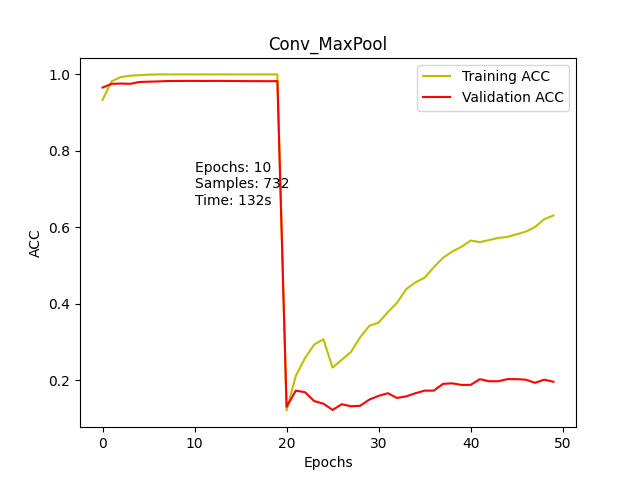
\includegraphics[height=5cm]{../../Plots/ba_plots/convmaxpool/2TFtr.png}
    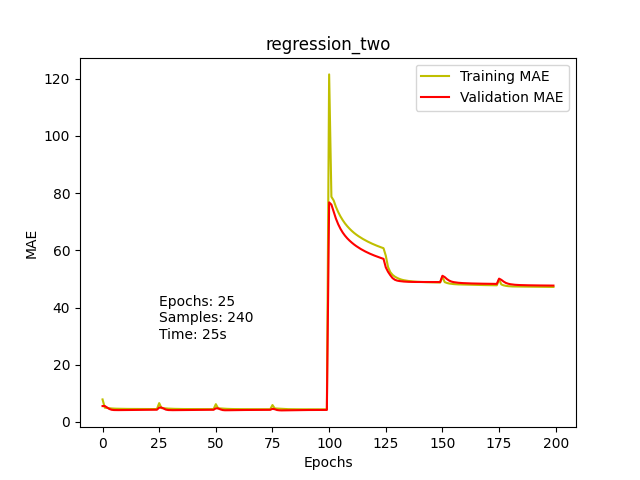
\includegraphics[height=5cm]{../../Plots/ba_plots/regr2/regr2train.png}
    \caption{\label{fig:ploterkl} 
    \small{Abgebildet sind exemplarische Plots zweier Deep-Cascade-Netzwerke – links für eine Klassifikationsaufgabe, rechts für eine 
    Regressionsaufgabe.
    Dargestellt werden die Tests CMP:TF2/732/10 und Regr2:TF4/240/25, die jeweils als typische Repräsentationen für den Einsatz von TF 
    in den entsprechenden Aufgabenbereichen dienen.}}
\end{figure}

Zur Erläuterung wird Abbildung \ref{fig:ploterkl} herangezogen. Die Überschriften der Plots sind die vollständigen Namen der dazugehörigen 
Netzwerke. In beiden Diagrammen sind jeweils drei Textzeilen angegeben, auf die im 
Folgenden näher eingegangen wird. Die erste Zeile gibt an, wie viele Trainings-Epochen pro Layer beziehungsweise Netzwerk durchgeführt wurden. 
Die zweite Zeile beschreibt, wie viele Trainingsbeispiele aus dem Trainingsdatensatz des Target-Datensatzes während des Trainings unter 
Verwendung von TF eingesetzt wurden. Die dritte Zeile gibt die gesamte Trainingsdauer in Sekunden an.

Im Fall der Klassifikation, bei der die Genauigkeit (Accuracy) von Interesse ist, wird die y-Achse mit "ACC" beschriftet, was auch im 
Funktionsnamen reflektiert wird. Ein Wert von 1 auf der y-Achse entspricht dabei einer Accuracy von 100\%. Abbildung 
\ref{fig:ploterkl} zeigt links ein Beispiel für diese Darstellungsweise.

Bei der Regression hingegen wird der mittlere absolute Fehler (MAE) betrachtet, welcher ebenfalls in der Bezeichnung der Funktionen sowie auf 
der y-Achse angegeben ist. Die y-Achse ist in Einheiten von 1000\$ pro Einheit skaliert. Hier gilt: Je niedriger der MAE-Wert, 
desto besser das Ergebnis.
